\subsection{Motor model}
A model of the motor needs to be made for the system model. The motor is a PMSM,  which means that it is driven by three phase currents. To simplify the model, the equivalent circuit for the d- and q-directions are drawn, and a model is made, based on those. In that way the PMSM can be controlled like an DC-machine.

\subsubsection{Motor model in the d-direction}
The equivalent circuit for the d-direction voltage $v_d$ of the PMSM is shown on figure \ref{fig:vd}.

\begin{figure}[H]
	\centering
	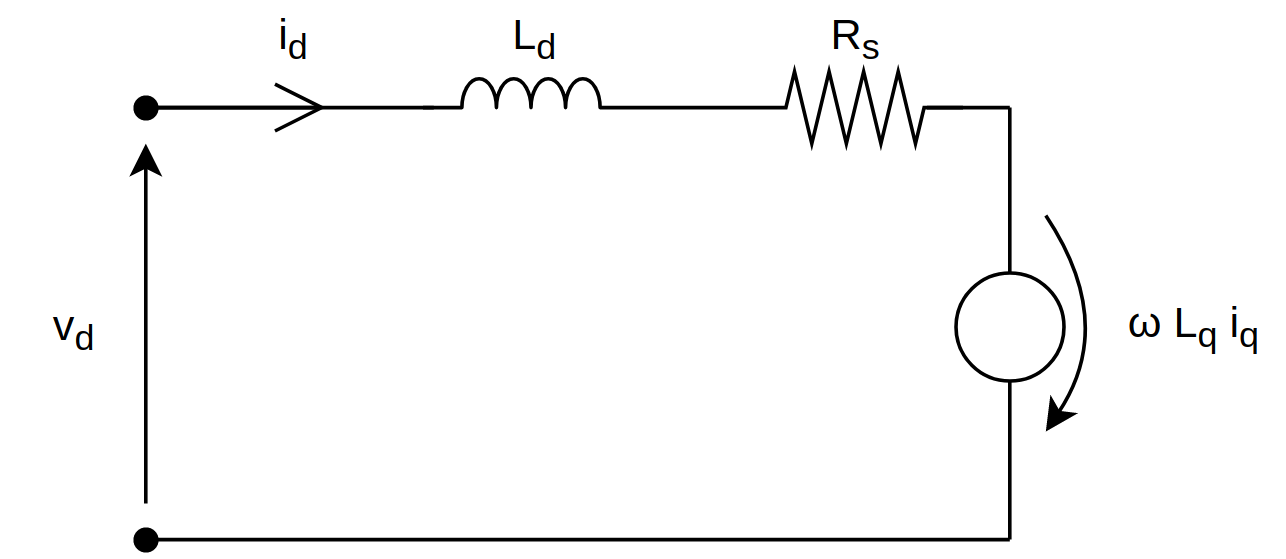
\includegraphics[width=0.6\linewidth]{pictures/control/vd}
	\caption{D-dierection equivalent circuit for the PMSM}
	\label{fig:vd}
\end{figure}


From the equivalent diagram the d-direction voltage can be described as in equation \ref{eq:d_direction}.

\begin{equation}
    \label{eq:d_direction}
    v_d = L_d \frac{d i_d}{dt} + R_s i_d - \omega L_q i_q
\end{equation}
% $\varphi_{rq} = L_qi_q$
% \begin{equation}\label{eq:d_direction2}
% v_{d} = \frac{d \varphi_{rq}}{dt} + R_s i_d - \omega \varphi_{rq}
% \end{equation}

$L_d$ and $L_q$ are respectively the d- and q-direction equivalent stator inductances for the motor, $i_d$ and $i_q$ are respectively the d- an q-direction currents, $R_s$ is the stator resistance for the motor, and $\omega$ is the rotational speed of the rotor.

If $i_d$ from the $L_d \frac{di_d}{dt}$ part is isolated and Laplace transformed it result in equation \ref{eq:d_direction}.

\begin{equation}
    \label{eq:d_direction2}
    I_d = \frac{1}{S} \frac{1}{L_d} (V_d - I_d R_d + \omega L_q I_q)
\end{equation}

From equation \ref{eq:d_direction2} the model of the d-direction of the motor is determined. That can be seen on figure \ref{fig:simulink_d_direction}.

\begin{figure}[H]
	\centering
	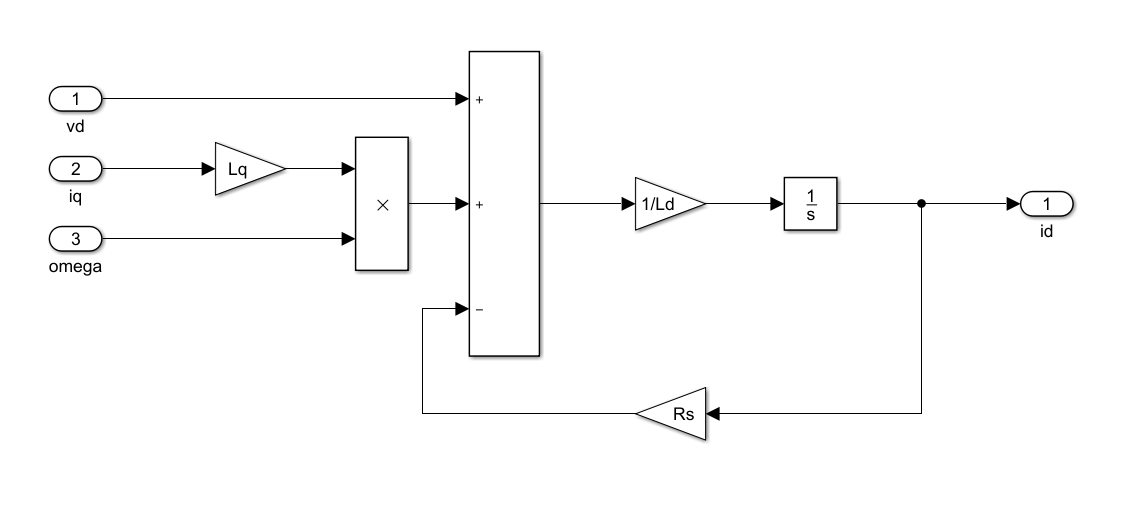
\includegraphics[width=0.8\linewidth]{pictures/control/simulink_d_direction.PNG}
	\caption{Simulink model of the d-direction of the motor model}
	\label{fig:simulink_d_direction}
\end{figure}



\subsubsection{Motor model in the q-direction}
The equivalent circuit for the q-direction voltage $v_q$ is shown on figure \ref{fig:vq}.

\begin{figure}[H]
	\centering
	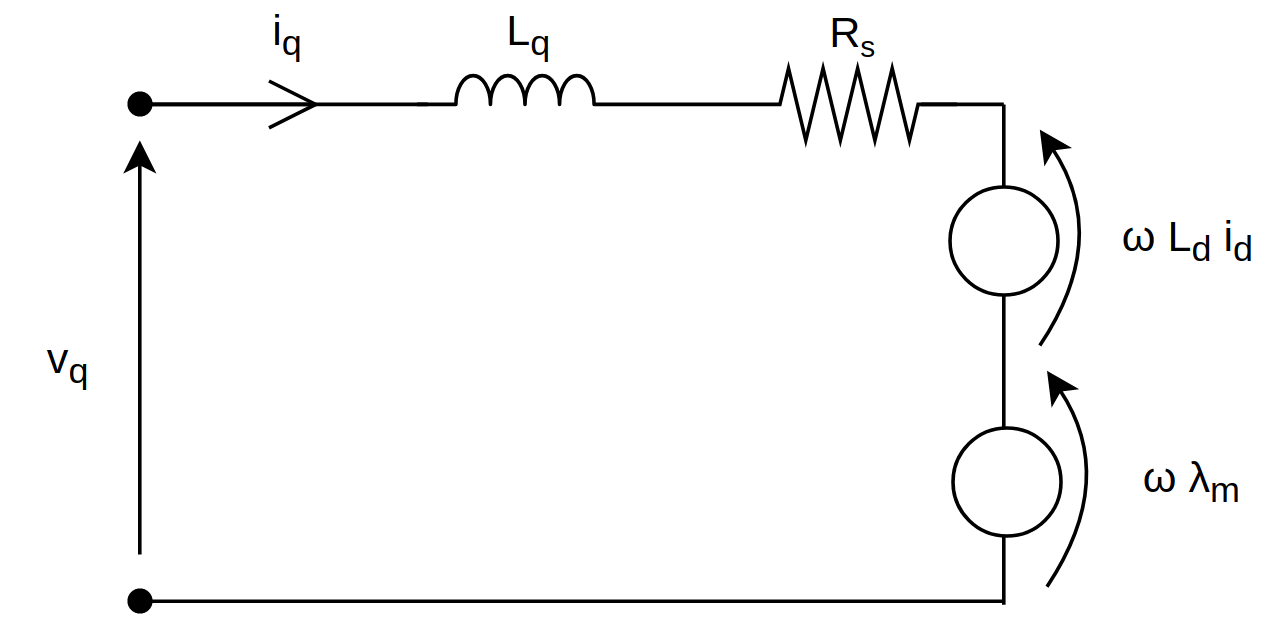
\includegraphics[width=0.6\linewidth]{pictures/control/vq.png}
	\caption{Q-direction equivalent circuit for the PMSM}
	\label{fig:vq}
\end{figure}

The voltage in the q-direction can be described from equation \ref{eq:q_direction}.

\begin{equation}
\label{eq:q_direction}
    v_q = L_q\frac{d i_q}{dt} + R_s i_q + \omega L_d i_d + \omega \lambda_m
\end{equation}

% \begin{equation}\label{eq:q_direction2}
% v_{sq} = R_si_q + \frac{d \varphi_{rd}}{dt} +  \omega_e \varphi_{rd}
% \end{equation}
% Where \\
% $\varphi_{rd} = L_di_d$

$\lambda_m$ is the flux linkage.

The $i_q$ from the $L_q \frac{di_q}{dt}$ part is isolated and Laplace transformed. This results in equation \ref{eq:d_direction}.

\begin{equation}
    \label{eq:q_direction2}
    I_q = \frac{1}{S} \frac{1}{L_q} (V_q - I_q R_q - \omega L_d I_d - \omega \lambda_m)
\end{equation}

From equation \ref{eq:q_direction2} the q-direction model can be produced. The model can be seen on figure \ref{fig:simulink_q_direction}.

\begin{figure}[H]
	\centering
	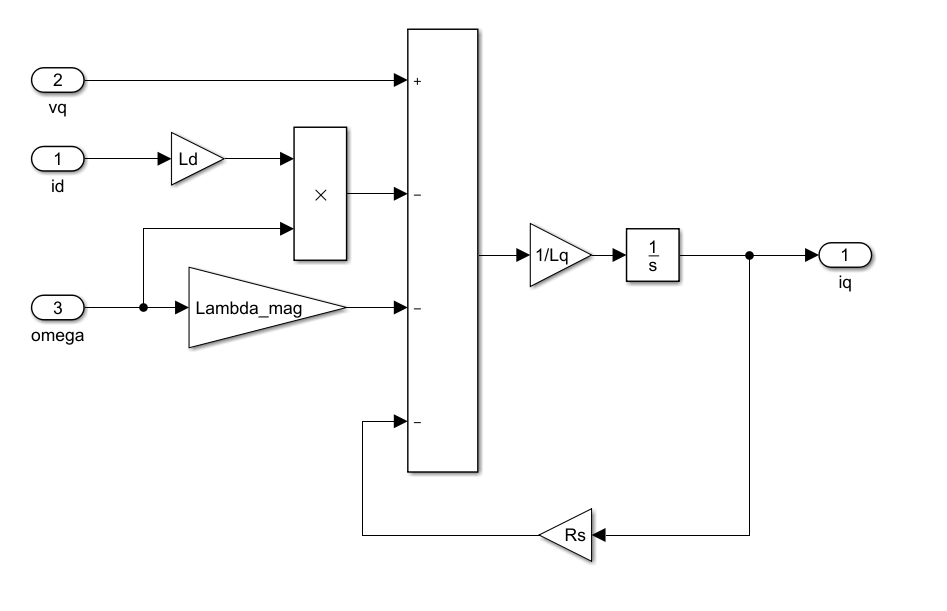
\includegraphics[width=0.8\linewidth]{pictures/control/simulink_q_direction.PNG}
	\caption{Simulink model of the q-direction of the motor model}
	\label{fig:simulink_q_direction}
\end{figure}


\subsubsection{Mechanical model}
For a multiple pole synchronous motor, the torque produced from the electrical field can be found from equation \ref{eq:torque_equation}.

\begin{equation}
    \label{eq:torque_equation}
    T_e = \frac{3P}{2} \big(\lambda_m i_{q} + (L_d - L_q) i_q i_{d}\big)
\end{equation}

Where $P$ is the number of pole pairs.

Because $L_q$ is higher than $L_d$, it can be seen from equation \ref{eq:torque_equation} the current running in the d-direction produces negative torque and is therefore reducing the output torque. 

The total torque at shaft of the motor, will be the sum of the torque the electrical field produces, the torque produces by the friction in the motor, and a possible external load torque. The total torque can be set equal to the inertia of the system multiplied with the acceleration. As seen in equation \ref{eq:total_torque}.

\begin{equation}
    \label{eq:total_torque}
    J\frac{d\omega}{dt} = T_e - B\omega - T_{load}
\end{equation}

$J$ is the inertia, $B$ is the friction coefficient, and $T_{load}$ is the torque from the external load.
Equation \ref{eq:total_torque} is rewritten and combined with equation \ref{eq:torque_equation} to a equation for the rotational speed. This is Laplace transformed, and the result is equation \ref{eq:omega}.

\begin{equation}
    \label{eq:omega}
    \omega = \frac{1}{S} \frac{1}{J} \bigg( \frac{3P}{2} \big( \lambda_m I_q + (L_d - L_q) I_q I_d \big) - B\omega - T_{load} \bigg)
\end{equation}

From equation \ref{eq:omega} can a model with the torque, rotational speed, and the angle of the motor as output, and the d- and q-current as inputs. This model can be seen on figure \ref{fig:torque}.

\begin{figure}[H]
	\centering
	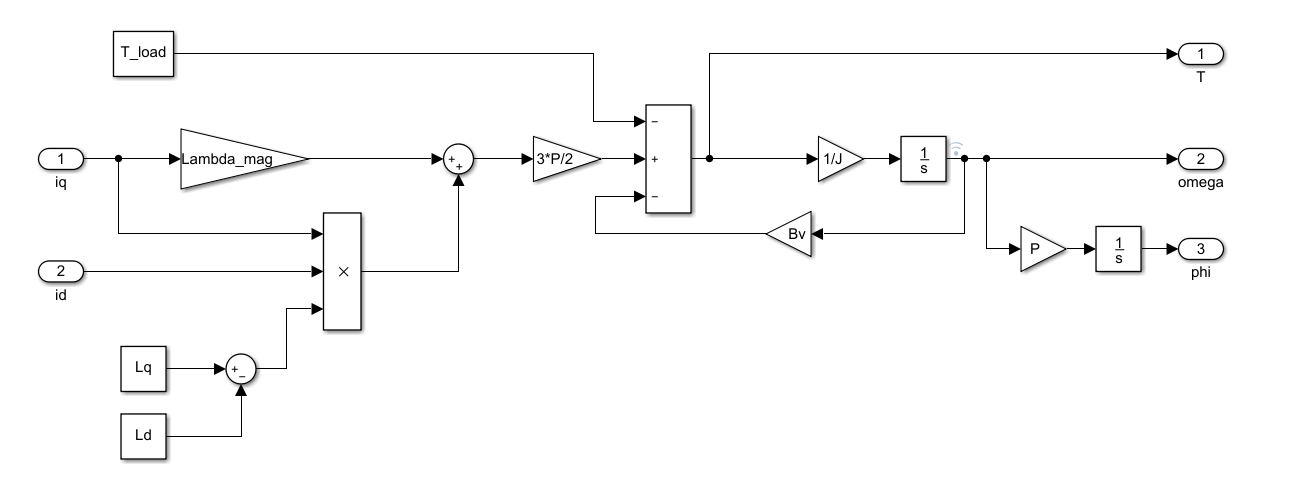
\includegraphics[width=1\linewidth]{pictures/control/torque.PNG}
	\caption{Simulink model of the motor with torque, rotational speed and the position of the rotor as output and the the d- and q-current as input}
	\label{fig:torque}
\end{figure}

\subsubsection{Complete motor model}
The three models, for the d-direction, the q-direction and the mechanical part, are put into subsystems and connected. This can be seen on figure \ref{fig:motor}

\begin{figure}[H]
	\centering
	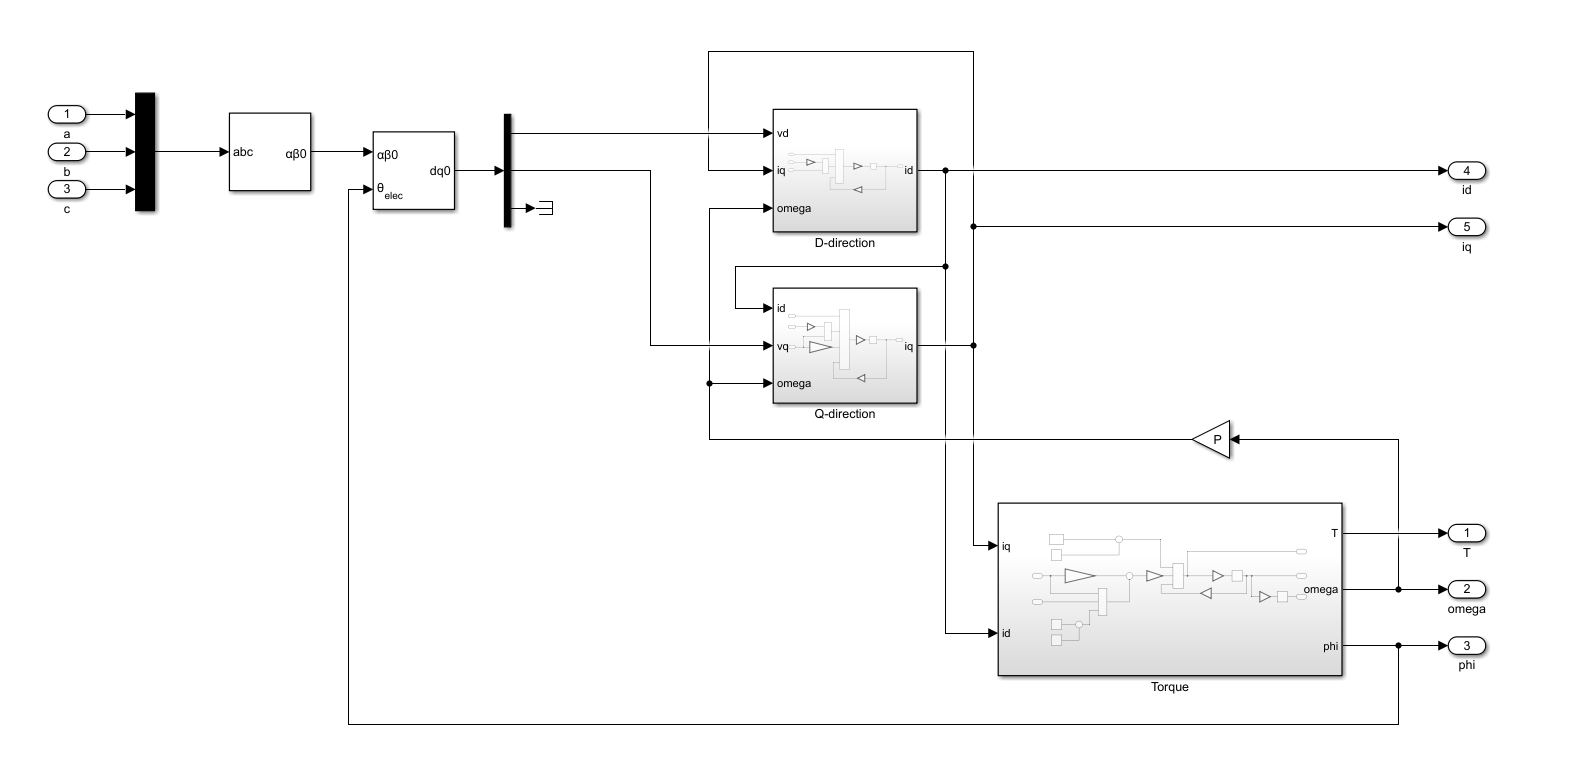
\includegraphics[width=1\linewidth]{pictures/control/motor_model.PNG}
	\caption{Simulink model of the full motor model}
	\label{fig:motor}
\end{figure}

Because the motor model is in the dq-frame, the three rotational phases voltages is converted to the dq-frame in the beginning of the model. The model outputs the d- and q-current, the torque, speed and angle of the motor. The rotational speed outputted from the motor model is the mechanical speed, and is therefore converted to the electrical speed before it is inputted to the d- and q-models. 